\documentclass[border=10pt]{standalone}
\usepackage[european]{circuitikz}
\usepackage{../../register-transfer-level}
\usetikzlibrary{shapes.geometric, arrows.meta, positioning, calc, shadows, decorations.markings}

\begin{document}

\begin{circuitikz}[>=Stealth, thick, line width=1.25]

	\node[rtl_module, rtl_width=30cm, rtl_height=1.5cm] at (0,0) (macroController) {\sffamily\LARGE Macro Pipeline Controller};

	\draw[->] (-16, -10) -- (-13.75, -10);
	\draw[->] (-16, -10.2)node[left]{\sffamily\LARGE PWM} -- (-13.95, -10.2);
	\draw[->] (-16, -10.4) -- (-14.15, -10.4);

	\node[rtl_module, rtl_width=3cm, rtl_height=8cm] at (-12, -10) () {};
	\node[rtl_reg] at (-11.0, -10.0) () {\sffamily\LARGE Reg};

	\node[rtl_module, rtl_width=3cm, rtl_height=8cm] at (-12.2, -10.2) () {};
	\node[rtl_reg] at (-11.2, -10.2) () {\sffamily\LARGE Reg};


	\node[rtl_module={\sffamily\LARGE Phase \\\sffamily\LARGE Sampler}, rtl_width=3cm, rtl_height=8cm] at (-12.4, -10.4) () {};
	\node[rtl_reg] at (-13.4, -10.4) () {\sffamily\LARGE Reg};
	\node[rtl_reg] at (-11.4, -10.4) () {\sffamily\LARGE Reg};


	\node[rtl_module={\sffamily\LARGE Magnitude \\\sffamily\LARGE Calculation}, rtl_width=3cm, rtl_height=6cm] at (-4, -6) () {};
	\node[rtl_reg] at (-3, -6) () {\sffamily\LARGE Reg};
	\node[rtl_reg] at (-5, -6) () {\sffamily\LARGE Reg};

	\node[rtl_module={\sffamily\LARGE Phase \\\sffamily\LARGE Calculation}, rtl_width=3cm, rtl_height=6cm] at (-4, -14) () {};
	\node[rtl_reg] at (-3, -14) () {\sffamily\LARGE Reg};
	\node[rtl_reg] at (-5, -14) () {\sffamily\LARGE Reg};

	\node[rtl_module={\sffamily\LARGE Magnitude \\\sffamily\LARGE Equalizer}, rtl_width=3cm, rtl_height=8cm] at (4, -8) () {};
	\node[rtl_reg] at (5, -8) () {\sffamily\LARGE Reg};
	\node[rtl_reg] at (3, -8) () {\sffamily\LARGE Reg};
	\node[rtl_reg] at (3, -10.5) () {\sffamily\LARGE Reg};

	\node[rtl_module={\sffamily\LARGE Output \\\sffamily\LARGE Module}, rtl_width=3cm, rtl_height=12cm] at (12, -10) () {};
	\node[rtl_reg] at (11, -8) () {\sffamily\LARGE Reg};
	\node[rtl_reg] at (13, -8) () {\sffamily\LARGE Reg};
	\node[rtl_reg] at (11, -14) () {\sffamily\LARGE Reg};
	\node[rtl_reg] at (13, -14) () {\sffamily\LARGE Reg};

	\draw[->] (-12.6, -0.75) -- (-12.6, -6) ;
	\draw[->] (-12.8, -0.75) -- (-12.8, -6.2);
	\draw[->] (-13, -0.75) node[left, above, rotate=90, xshift=-1.15cm] {\sffamily\LARGE START} -- (-13, -6.4); %edge-0.4cm -> center +0.6cm

	\draw[->] (-11.4, -6) -- (-11.4, -0.75) node[left, below, rotate=90, xshift=-1.15cm] {\sffamily\LARGE BUSY};
	\draw[->] (-11.6, -6.2) -- (-11.6, -0.75);
	\draw[->] (-11.8, -6.4) -- (-11.8, -0.75);

	\draw[->] (-4.6, -0.75) node[left, above, rotate=90, xshift=-1.15cm] {\sffamily\LARGE START} -- (-4.6, -3);
	\draw[->] (-3.4, -3) -- (-3.4, -0.75)node[left, below, rotate=90, xshift=-1.15cm] {\sffamily\LARGE BUSY};

	\draw[->] (-0.6, -0.75) node[left, above, rotate=90, xshift=-1.15cm] {\sffamily\LARGE START} -- (-0.6, -9.7) -- (-4.6, -9.7) -- (-4.6, -11);
	\draw[->] (-3.4, -11) -- (-3.4,-10.3) -- (0.6, -10.3) -- (0.6, -0.75)node[left, below, rotate=90, xshift=-1.15cm] {\sffamily\LARGE BUSY};

	\draw[->] (3.4, -0.75) node[left, above, rotate=90, xshift=-1.15cm] {\sffamily\LARGE START} -- (3.4, -4);
	\draw[->] (4.6, -4) -- (4.6, -0.75) node[left, below, rotate=90, xshift=-1.15cm] {\sffamily\LARGE BUSY};

	\draw[->] (11.4, -0.75) node[left, above, rotate=90, xshift=-1.15cm] {\sffamily\LARGE START} -- (11.4, -4);
	\draw[->] (12.6, -4) -- (12.6, -0.75) node[left, below, rotate=90, xshift=-1.15cm] {\sffamily\LARGE BUSY};

	\draw[-, rtl_bus, line width=3] (-10.25, -10.0) -- (-8.9, -10.0);
	\node[circ] at (-8.9, -10) (pwmWNode) {};
	\draw[->, line width=3] (pwmWNode) -- (-8.9, -6.4) -- (-5.75, -6.4);
	\draw[->, line width=3] (pwmWNode) -- (-8.9, -13.6) -- (-5.75, -13.6);

	\draw[-,rtl_bus, line width=3] (-10.45, -10.2) -- (-9.3, -10.2) node[midway, xshift=2cm]{\sffamily\LARGE $\mathsf{D_{u,v,w}}$};
	\node[circ] at (-9.3, -10.2) (pwmVNode) {};
	\draw[->, line width=3] (pwmVNode) -- (-9.3, -6) -- (-5.75, -6);
	\draw[->, line width=3] (pwmVNode) -- (-9.3, -14) -- (-5.75, -14);

	\draw[-, rtl_bus, line width=3] (-10.65, -10.4) -- (-9.7, -10.4);
	\node[circ] at (-9.7, -10.4) (pwmUNode) {};
	\draw[->, line width=3] (pwmUNode) -- (-9.7, -5.6) -- (-5.75, -5.6);
	\draw[->, line width=3] (pwmUNode) -- (-9.7, -14.4) -- (-5.75, -14.4) ;

	\draw[->, rtl_bus, line width=3] (-2.25, -6) -- (0, -6) node[above, midway, yshift=0.15cm, xshift=-0.15cm]{\sffamily\LARGE $\mathsf{||\vec{v}||_{2}}$} -- (0, -8)  -- (2.25, -8) ;

	\draw[->, rtl_bus, line width=3] (5.75, -8) -- (10.25, -8) node[above, midway, yshift=0.15cm]{\sffamily\LARGE $\mathsf{\hat{v}}$};
	\draw[->, rtl_bus, line width=3] (-2.25, -14) -- (10.25, -14)node[above, midway, yshift=0.15cm]{\sffamily\LARGE $\mathsf{\phi}$};
	\node[circ, fill=black, scale=2] at (1, -14) (phaseNode) {};
	\draw[->, line width=3] (phaseNode) -- +(0, 3.5) -- +(1.25, 3.5);


	\draw[->, rtl_bus, line width=3] (13.75, -8) -- (16, -8) node[right] {\Huge $\mathsf{\hat{v}}$};
	\draw[->, rtl_bus, line width=3] (13.75, -14) -- (16, -14) node[right] {\Huge $\mathsf{\phi}$};

	\node[]at (3, -26.5) (core2) {
		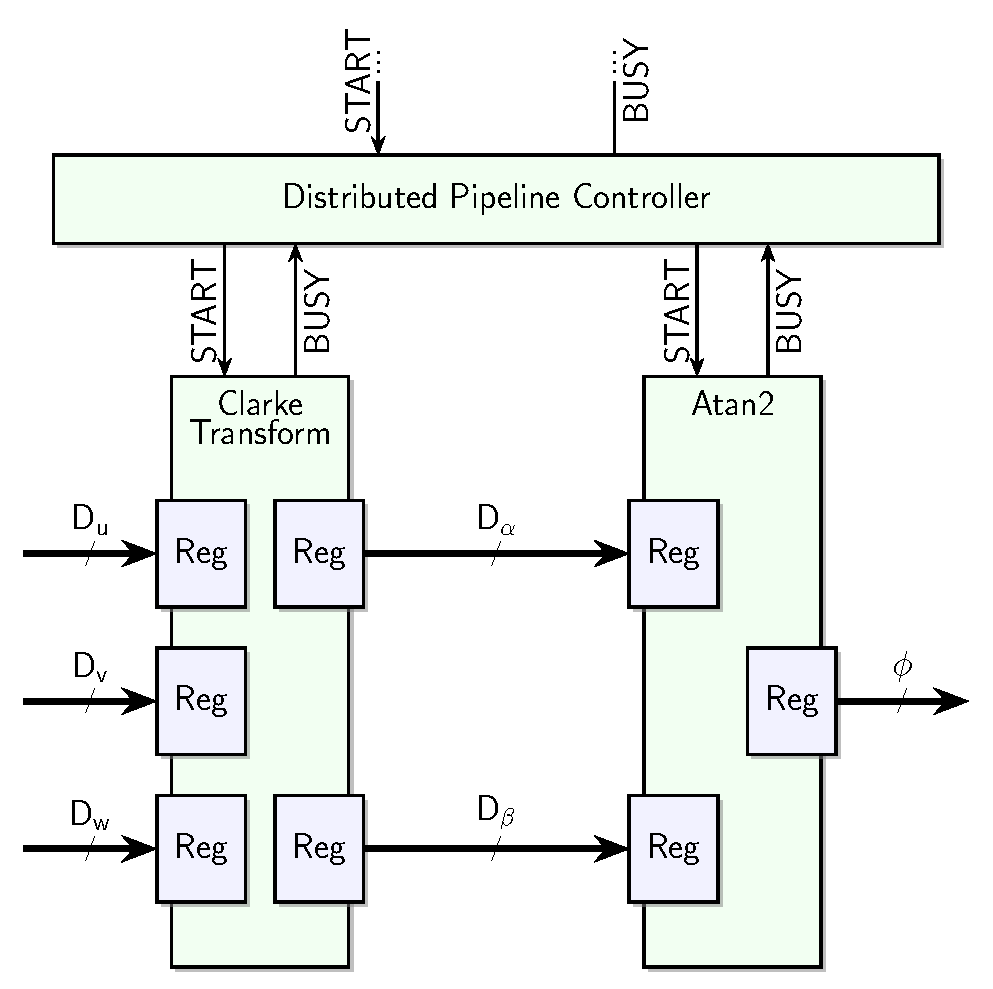
\includegraphics[width=18cm, height=16cm]{Distributed_Pipeline.pdf}
	};

	\draw[dashed, line width=2.5] (-4, -14) circle (4) ;
	\draw[->, dashed, line width = 2.5] (-4,-18) -- (-3, -20);

	\node[]at (40, -20) (core2) {
		
\includegraphics[width=45cm, height=28cm]{CORDIC_Pipeline.pdf}
	};

	\draw[dashed, line width=2.5] (7.4, -29.45) circle (6) ;
	\draw[->, dashed, line width = 2.5] (13.4,-29.45) -- (19, -22);
\end{circuitikz}
\end{document}
